\documentclass{article}

\usepackage{fancyhdr}
\usepackage{extramarks}
\usepackage{amsmath}
\usepackage{amsthm}
\usepackage{amsfonts}
\usepackage{tikz}
\usepackage[shortlabels]{enumitem}
\usepackage{mathtools}
\usepackage{amssymb}

\usetikzlibrary{automata,positioning}

%
% Basic Document Settings
%

\topmargin=-0.45in
\evensidemargin=0in
\oddsidemargin=0in
\textwidth=6.5in
\textheight=9.0in
\headsep=0.25in

\linespread{1.1}

\pagestyle{fancy}
\lhead{\hmwkAuthorName}
\chead{\hmwkClass\ (\hmwkClassInstructor\ \hmwkClassTime): \hmwkTitle}
\lfoot{\lastxmark}
\cfoot{\thepage}

\renewcommand\headrulewidth{0.4pt}
\renewcommand\footrulewidth{0.4pt}

\setlength\parindent{0pt}

%
% Create Problem Sections
%

\newcommand{\enterProblemHeader}[1]{
    \nobreak\extramarks{}{Problem \arabic{#1} continued on next page\ldots}\nobreak{}
    \nobreak\extramarks{Problem \arabic{#1} (continued)}{Problem \arabic{#1} continued on next page\ldots}\nobreak{}
}

\newcommand{\exitProblemHeader}[1]{
    \nobreak\extramarks{Problem \arabic{#1} (continued)}{Problem \arabic{#1} continued on next page\ldots}\nobreak{}
    \stepcounter{#1}
    \nobreak\extramarks{Problem \arabic{#1}}{}\nobreak{}
}

\setcounter{secnumdepth}{0}
\newcounter{partCounter}
\newcounter{homeworkProblemCounter}
\setcounter{homeworkProblemCounter}{1}
\nobreak\extramarks{Problem \arabic{homeworkProblemCounter}}{}\nobreak{}

\newcommand{\hmwkTitle}{Mod 2}
\newcommand{\hmwkDueDate}{February 20, 2025}
\newcommand{\hmwkClass}{Discrete Math}
\newcommand{\hmwkClassTime}{Section 001}
\newcommand{\hmwkClassInstructor}{Mark Floryan}
\newcommand{\hmwkAuthorName}{\textbf{Rushil Umaretiya}}

%
% Title Page
%

\title{
    \vspace{2in}
    \textmd{\textbf{\hmwkTitle}}\\
    \normalsize\vspace{0.1in}
    \small{\textbf{Due\ on\ \hmwkDueDate}}\\
    \normalsize\text{Tuesday/Thursday 11:00-12:15, Warner 209}\\
    \vspace{0.1in}\large{\textit{\hmwkClassInstructor\ - \hmwkClassTime}}
    \vspace{3in}
}

\author{\hmwkAuthorName\\\small{frj2ka@virginia.edu}}
\date{}

\renewcommand{\part}[1]{\textbf{\large Part \Alph{partCounter}}\stepcounter{partCounter}\\}

%
% Various Helper Commands
%

% Useful for algorithms
\newcommand{\alg}[1]{\textsc{\bfseries \footnotesize #1}}

% For derivatives
\newcommand{\deriv}[1]{\frac{\mathrm{d}}{\mathrm{d}x} (#1)}

% For partial derivatives
\newcommand{\pderiv}[2]{\frac{\partial}{\partial #1} (#2)}

% Integral dx
\newcommand{\dx}{\mathrm{d}x}

% Alias for the Solution section header
\newcommand{\solution}{\textbf{\large Solution}}

\newcommand{\unit}[1]{\section{Unit #1}}
\newcommand{\problem}[1]{\textbf{\##1}}
\newcommand{\prob}[1]{\problem{#1}}


% Probability commands: Expectation, Variance, Covariance, Bias
\newcommand{\E}{\mathrm{E}}
\newcommand{\Var}{\mathrm{Var}}
\newcommand{\Cov}{\mathrm{Cov}}
\newcommand{\Bias}{\mathrm{Bias}}

\renewcommand{\And}{\wedge}
\newcommand{\Or}{\vee}
\newcommand{\Xor}{\oplus}
\newcommand{\Not}{\neg}
\newcommand{\Implies}{\rightarrow}
\newcommand{\Iff}{\leftrightarrow}
\newcommand{\union}{\cup}
\newcommand{\intersection}{\cap}

\newcommand{\AllIntegers}{\mathbb{Z}}
\newcommand{\AllNaturals}{\mathbb{N}}
\newcommand{\AllRationals}{\mathbb{Q}}
\newcommand{\AllReals}{\mathbb{R}}
\newcommand{\AllComplexes}{\mathbb{C}}

\begin{document}

\maketitle

\pagebreak

\problem{1} Draw out \emph{DFA}s (not \emph{NFA}s) for each of the following languages. For some of these, a small hint is provided. Your goal is to construct a \emph{DFA} with as few states as possible (just like how we prefer to write succinct code when possible). For all of these, let $\Sigma = \{a,b\}$

\begin{itemize}
	\item $\{w \ | \ w \text{ does not contain the substring } abba \}$ (\emph{*Hint: Draw out the DFA for a simpler language that DOES contain abba and then try to change that machine slightly.})
	

\begin{center}
    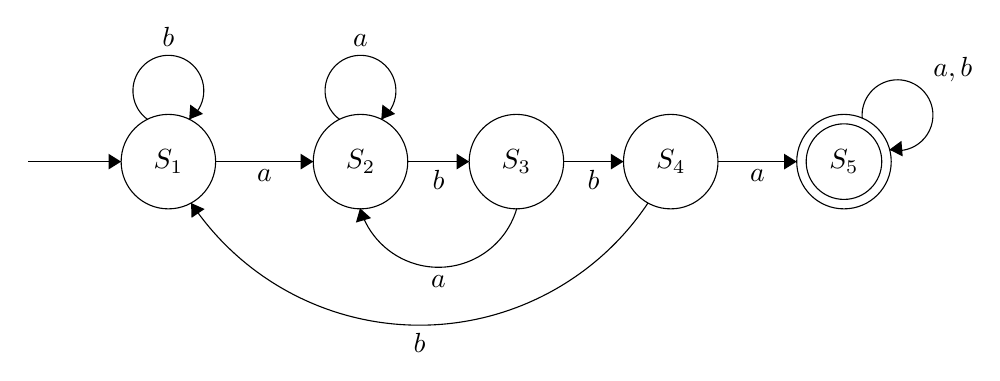
\begin{tikzpicture}[scale=0.2]
    \tikzstyle{every node}+=[inner sep=0pt]
    \draw [black] (14.4,-22.3) circle (3);
    \draw (14.4,-22.3) node {$S_1$};
    \draw [black] (26.6,-22.3) circle (3);
    \draw (26.6,-22.3) node {$S_2$};
    \draw [black] (36.5,-22.3) circle (3);
    \draw (36.5,-22.3) node {$S_3$};
    \draw [black] (46.3,-22.3) circle (3);
    \draw (46.3,-22.3) node {$S_4$};
    \draw [black] (57.3,-22.3) circle (3);
    \draw (57.3,-22.3) node {$S_5$};
    \draw [black] (57.3,-22.3) circle (2.4);
    \draw [black] (5.5,-22.3) -- (11.4,-22.3);
    \fill [black] (11.4,-22.3) -- (10.6,-21.8) -- (10.6,-22.8);
    \draw [black] (13.077,-19.62) arc (234:-54:2.25);
    \draw (14.4,-15.05) node [above] {$b$};
    \fill [black] (15.72,-19.62) -- (16.6,-19.27) -- (15.79,-18.68);
    \draw [black] (17.4,-22.3) -- (23.6,-22.3);
    \fill [black] (23.6,-22.3) -- (22.8,-21.8) -- (22.8,-22.8);
    \draw (20.5,-22.8) node [below] {$a$};
    \draw [black] (29.6,-22.3) -- (33.5,-22.3);
    \fill [black] (33.5,-22.3) -- (32.7,-21.8) -- (32.7,-22.8);
    \draw (31.55,-22.8) node [below] {$b$};
    \draw [black] (39.5,-22.3) -- (43.3,-22.3);
    \fill [black] (43.3,-22.3) -- (42.5,-21.8) -- (42.5,-22.8);
    \draw (41.4,-22.8) node [below] {$b$};
    \draw [black] (49.3,-22.3) -- (54.3,-22.3);
    \fill [black] (54.3,-22.3) -- (53.5,-21.8) -- (53.5,-22.8);
    \draw (51.8,-22.8) node [below] {$a$};
    \draw [black] (36.529,-25.258) arc (-16.02213:-163.97787:5.181);
    \fill [black] (26.57,-25.26) -- (26.31,-26.17) -- (27.27,-25.89);
    \draw (31.55,-29.51) node [below] {$a$};
    \draw [black] (25.277,-19.62) arc (234:-54:2.25);
    \draw (26.6,-15.05) node [above] {$a$};
    \fill [black] (27.92,-19.62) -- (28.8,-19.27) -- (27.99,-18.68);
    \draw [black] (44.857,-24.926) arc (-33.71015:-146.28985:17.44);
    \fill [black] (15.84,-24.93) -- (15.87,-25.87) -- (16.7,-25.31);
    \draw (30.35,-33.19) node [below] {$b$};
    \draw [black] (58.459,-19.546) arc (184.91438:-103.08562:2.25);
    \draw (62.95,-16.43) node [right] {$a,b$};
    \fill [black] (60.19,-21.54) -- (61.03,-21.97) -- (60.95,-20.98);
    \end{tikzpicture}
    \end{center}


	\item $\{w \ | \ w \text{ contains BOTH the substrings ab and ba}\}$
	

    \begin{center}
        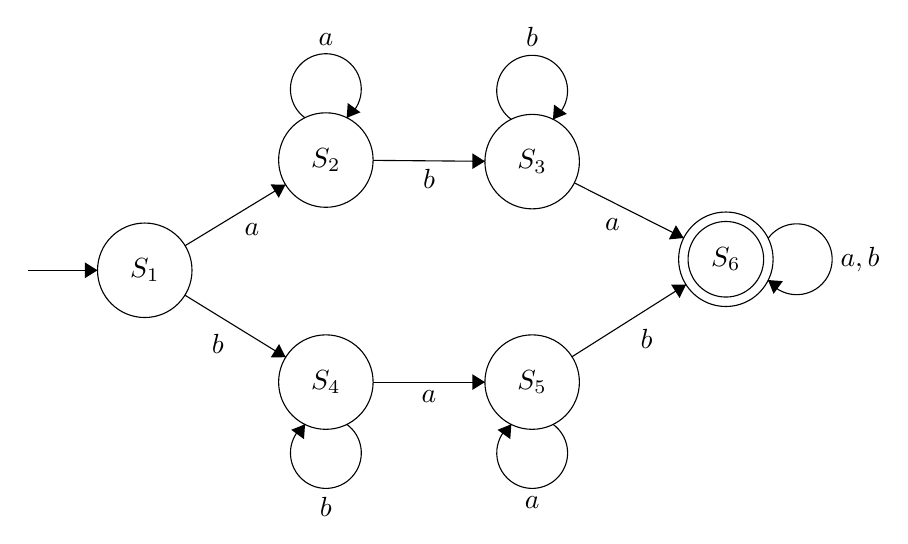
\begin{tikzpicture}[scale=0.2]
        \tikzstyle{every node}+=[inner sep=0pt]
        \draw [black] (12.7,-30.3) circle (3);
        \draw (12.7,-30.3) node {$S_1$};
        \draw [black] (24.2,-23.3) circle (3);
        \draw (24.2,-23.3) node {$S_2$};
        \draw [black] (37.3,-23.4) circle (3);
        \draw (37.3,-23.4) node {$S_3$};
        \draw [black] (24.2,-37.4) circle (3);
        \draw (24.2,-37.4) node {$S_4$};
        \draw [black] (37.3,-37.4) circle (3);
        \draw (37.3,-37.4) node {$S_5$};
        \draw [black] (49.6,-29.6) circle (3);
        \draw (49.6,-29.6) node {$S_6$};
        \draw [black] (49.6,-29.6) circle (2.4);
        \draw [black] (5.3,-30.3) -- (9.7,-30.3);
        \fill [black] (9.7,-30.3) -- (8.9,-29.8) -- (8.9,-30.8);
        \draw [black] (15.26,-28.74) -- (21.64,-24.86);
        \fill [black] (21.64,-24.86) -- (20.69,-24.85) -- (21.21,-25.7);
        \draw (19.51,-27.3) node [below] {$a$};
        \draw [black] (27.2,-23.32) -- (34.3,-23.38);
        \fill [black] (34.3,-23.38) -- (33.5,-22.87) -- (33.5,-23.87);
        \draw (30.75,-23.86) node [below] {$b$};
        \draw [black] (39.98,-24.75) -- (46.92,-28.25);
        \fill [black] (46.92,-28.25) -- (46.43,-27.44) -- (45.98,-28.34);
        \draw (42.4,-27) node [below] {$a$};
        \draw [black] (15.25,-31.88) -- (21.65,-35.82);
        \fill [black] (21.65,-35.82) -- (21.23,-34.98) -- (20.7,-35.83);
        \draw (17.34,-34.35) node [below] {$b$};
        \draw [black] (27.2,-37.4) -- (34.3,-37.4);
        \fill [black] (34.3,-37.4) -- (33.5,-36.9) -- (33.5,-37.9);
        \draw (30.75,-37.9) node [below] {$a$};
        \draw [black] (39.83,-35.79) -- (47.07,-31.21);
        \fill [black] (47.07,-31.21) -- (46.12,-31.21) -- (46.66,-32.06);
        \draw (44.56,-34) node [below] {$b$};
        \draw [black] (22.877,-20.62) arc (234:-54:2.25);
        \draw (24.2,-16.05) node [above] {$a$};
        \fill [black] (25.52,-20.62) -- (26.4,-20.27) -- (25.59,-19.68);
        \draw [black] (35.977,-20.72) arc (234:-54:2.25);
        \draw (37.3,-16.15) node [above] {$b$};
        \fill [black] (38.62,-20.72) -- (39.5,-20.37) -- (38.69,-19.78);
        \draw [black] (25.523,-40.08) arc (54:-234:2.25);
        \draw (24.2,-44.65) node [below] {$b$};
        \fill [black] (22.88,-40.08) -- (22,-40.43) -- (22.81,-41.02);
        \draw [black] (38.623,-40.08) arc (54:-234:2.25);
        \draw (37.3,-44.65) node [below] {$a$};
        \fill [black] (35.98,-40.08) -- (35.1,-40.43) -- (35.91,-41.02);
        \draw [black] (52.28,-28.277) arc (144:-144:2.25);
        \draw (56.85,-29.6) node [right] {$a,b$};
        \fill [black] (52.28,-30.92) -- (52.63,-31.8) -- (53.22,-30.99);
        \end{tikzpicture}
        \end{center}

	\item $\{w \ | \ w \in a^*b^*a^* \}$
	
    
\begin{center}
    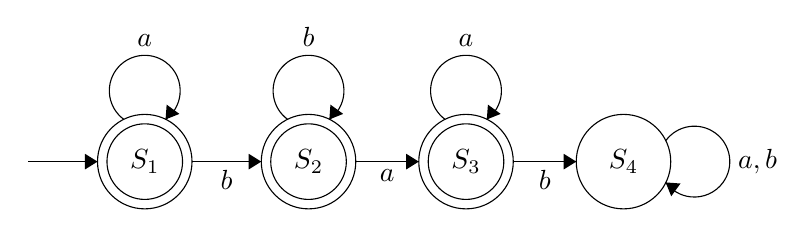
\begin{tikzpicture}[scale=0.2]
    \tikzstyle{every node}+=[inner sep=0pt]
    \draw [black] (13.5,-30.3) circle (3);
    \draw (13.5,-30.3) node {$S_1$};
    \draw [black] (13.5,-30.3) circle (2.4);
    \draw [black] (23.9,-30.3) circle (3);
    \draw (23.9,-30.3) node {$S_2$};
    \draw [black] (23.9,-30.3) circle (2.4);
    \draw [black] (33.9,-30.3) circle (3);
    \draw (33.9,-30.3) node {$S_3$};
    \draw [black] (33.9,-30.3) circle (2.4);
    \draw [black] (43.9,-30.3) circle (3);
    \draw (43.9,-30.3) node {$S_4$};
    \draw [black] (6.1,-30.3) -- (10.5,-30.3);
    \fill [black] (10.5,-30.3) -- (9.7,-29.8) -- (9.7,-30.8);
    \draw [black] (16.5,-30.3) -- (20.9,-30.3);
    \fill [black] (20.9,-30.3) -- (20.1,-29.8) -- (20.1,-30.8);
    \draw (18.7,-30.8) node [below] {$b$};
    \draw [black] (26.9,-30.3) -- (30.9,-30.3);
    \fill [black] (30.9,-30.3) -- (30.1,-29.8) -- (30.1,-30.8);
    \draw (28.9,-30.8) node [below] {$a$};
    \draw [black] (36.9,-30.3) -- (40.9,-30.3);
    \fill [black] (40.9,-30.3) -- (40.1,-29.8) -- (40.1,-30.8);
    \draw (38.9,-30.8) node [below] {$b$};
    \draw [black] (22.577,-27.62) arc (234:-54:2.25);
    \draw (23.9,-23.05) node [above] {$b$};
    \fill [black] (25.22,-27.62) -- (26.1,-27.27) -- (25.29,-26.68);
    \draw [black] (32.577,-27.62) arc (234:-54:2.25);
    \draw (33.9,-23.05) node [above] {$a$};
    \fill [black] (35.22,-27.62) -- (36.1,-27.27) -- (35.29,-26.68);
    \draw [black] (46.58,-28.977) arc (144:-144:2.25);
    \draw (51.15,-30.3) node [right] {$a,b$};
    \fill [black] (46.58,-31.62) -- (46.93,-32.5) -- (47.52,-31.69);
    \draw [black] (12.177,-27.62) arc (234:-54:2.25);
    \draw (13.5,-23.05) node [above] {$a$};
    \fill [black] (14.82,-27.62) -- (15.7,-27.27) -- (14.89,-26.68);
    \end{tikzpicture}
    \end{center}

    \pagebreak

	\item $\{w \ | \ w \neq ab \wedge w \neq bb \}$
	

\begin{center}
    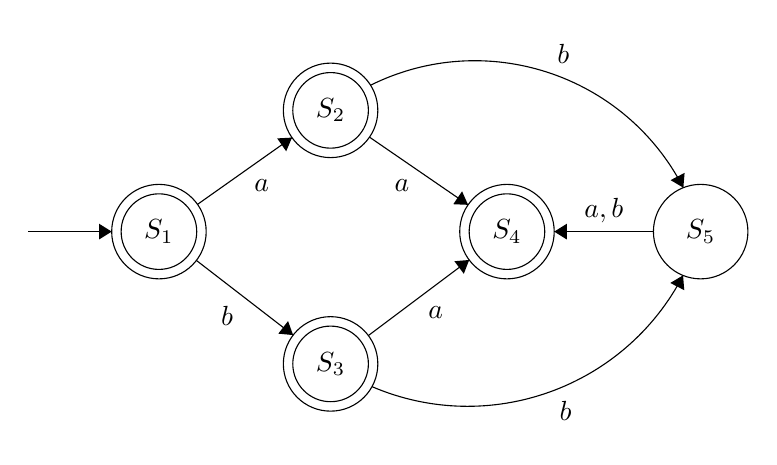
\begin{tikzpicture}[scale=0.2]
    \tikzstyle{every node}+=[inner sep=0pt]
    \draw [black] (13,-30.2) circle (3);
    \draw (13,-30.2) node {$S_1$};
    \draw [black] (13,-30.2) circle (2.4);
    \draw [black] (23.9,-22.5) circle (3);
    \draw (23.9,-22.5) node {$S_2$};
    \draw [black] (23.9,-22.5) circle (2.4);
    \draw [black] (23.9,-38.6) circle (3);
    \draw (23.9,-38.6) node {$S_3$};
    \draw [black] (23.9,-38.6) circle (2.4);
    \draw [black] (35.1,-30.2) circle (3);
    \draw (35.1,-30.2) node {$S_4$};
    \draw [black] (35.1,-30.2) circle (2.4);
    \draw [black] (47.4,-30.2) circle (3);
    \draw (47.4,-30.2) node {$S_5$};
    \draw [black] (15.45,-28.47) -- (21.45,-24.23);
    \fill [black] (21.45,-24.23) -- (20.51,-24.28) -- (21.08,-25.1);
    \draw (19.52,-26.85) node [below] {$a$};
    \draw [black] (15.38,-32.03) -- (21.52,-36.77);
    \fill [black] (21.52,-36.77) -- (21.2,-35.88) -- (20.58,-36.68);
    \draw (17.33,-34.9) node [below] {$b$};
    \draw [black] (26.37,-24.2) -- (32.63,-28.5);
    \fill [black] (32.63,-28.5) -- (32.25,-27.64) -- (31.69,-28.46);
    \draw (28.43,-26.85) node [below] {$a$};
    \draw [black] (26.3,-36.8) -- (32.7,-32);
    \fill [black] (32.7,-32) -- (31.76,-32.08) -- (32.36,-32.88);
    \draw (30.57,-34.9) node [below] {$a$};
    \draw [black] (46.284,-32.98) arc (-27.44648:-113.21498:15.417);
    \fill [black] (46.28,-32.98) -- (45.47,-33.46) -- (46.36,-33.92);
    \draw (38.82,-40.92) node [below] {$b$};
    \draw [black] (26.435,-20.905) arc (116.41745:27.29879:14.897);
    \fill [black] (46.3,-27.41) -- (46.38,-26.47) -- (45.49,-26.93);
    \draw (38.68,-19.55) node [above] {$b$};
    \draw [black] (44.4,-30.2) -- (38.1,-30.2);
    \fill [black] (38.1,-30.2) -- (38.9,-30.7) -- (38.9,-29.7);
    \draw (41.25,-29.7) node [above] {$a,b$};
    \draw [black] (4.7,-30.2) -- (10,-30.2);
    \fill [black] (10,-30.2) -- (9.2,-29.7) -- (9.2,-30.7);
    \end{tikzpicture}
    \end{center}
    

	\item $\{w \ | \ w \in a^iw' \ | \ i \in \mathbb{N}, w' \in \{a,b\}^*, \text{w' contains at least i a's}\} $ (\emph{*Hint: This one LOOKS not regular but it actually is. Can you figure out why?})
	
    \textbf{Note: }This will accept everything due to the $w'$.
	
    \begin{center}
        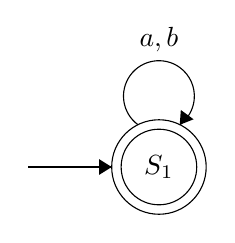
\begin{tikzpicture}[scale=0.2]
        \tikzstyle{every node}+=[inner sep=0pt]
        \draw [black] (13,-30.2) circle (3);
        \draw (13,-30.2) node {$S_1$};
        \draw [black] (13,-30.2) circle (2.4);
        \draw [black] (4.7,-30.2) -- (10,-30.2);
        \fill [black] (10,-30.2) -- (9.2,-29.7) -- (9.2,-30.7);
        \draw [black] (11.677,-27.52) arc (234:-54:2.25);
        \draw (13,-22.95) node [above] {$a,b$};
        \fill [black] (14.32,-27.52) -- (15.2,-27.17) -- (14.39,-26.58);
        \end{tikzpicture}
        \end{center}
\end{itemize}

\pagebreak

\problem{2} Prove that regular languages are closed under \emph{intersection}. Do this by starting with \emph{DFA}s for two regular languages $A$ and $B$, and describe how to construct a new \emph{DFA} for $A \cap B$

\begin{proof}
    Let $A$ and $B$ be regular languages. Let $M_A = (Q_A, \Sigma, \delta_A, q_{0A}, F_A)$ and $M_B = (Q_B, \Sigma, \delta_B, q_{0B}, F_B)$ be the \emph{DFA}s that recognize $A$ and $B$ respectively. We will construct a new \emph{DFA} $M = (Q, \Sigma, \delta, q_0, F)$ that recognizes $A \cap B$.\\

    Let
    \begin{align*}
        Q &= Q_A \times Q_B\\
        \delta((q_A, q_B), a) &= (\delta_A(q_A, a), \delta_B(q_B, a))\\
        q_0 &= (q_{0A}, q_{0B})\\
        F &= F_A \times F_B
    \end{align*}
    
    Let $w \in A \cap B$. Then $w \in A$ and $w \in B$. Since $M_A$ and $M_B$ recognize $A$ and $B$ respectively, $M_A$ will accept $w$ and $M_B$ will accept $w$. Thus, $M$ will accept $w$ as well. Thus, $A \cap B$ is regular.
\end{proof}

An alternative way to prove that regular languages are closed under intersection is to acknowledge that since regular languages can be represented by NFAs, we can create an NFA to represent the unison of the two languages.

\begin{center}
    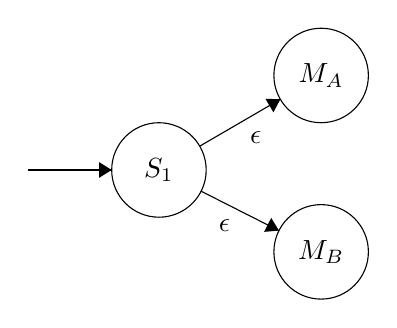
\begin{tikzpicture}[scale=0.2]
    \tikzstyle{every node}+=[inner sep=0pt]
    \draw [black] (19.8,-33.8) circle (3);
    \draw (19.8,-33.8) node {$S_1$};
    \draw [black] (30.1,-27.8) circle (3);
    \draw (30.1,-27.8) node {$M_A$};
    \draw [black] (30.1,-39) circle (3);
    \draw (30.1,-39) node {$M_B$};
    \draw [black] (11.5,-33.8) -- (16.8,-33.8);
    \fill [black] (16.8,-33.8) -- (16,-33.3) -- (16,-34.3);
    \draw [black] (22.39,-32.29) -- (27.51,-29.31);
    \fill [black] (27.51,-29.31) -- (26.56,-29.28) -- (27.07,-30.14);
    \draw (25.94,-31.3) node [below] {$\epsilon$};
    \draw [black] (22.48,-35.15) -- (27.42,-37.65);
    \fill [black] (27.42,-37.65) -- (26.93,-36.84) -- (26.48,-37.73);
    \draw (23.96,-36.9) node [below] {$\epsilon$};
    \end{tikzpicture}
\end{center}

In this diagram, $S_1$ is the start state, $M_A$ is the NFA that recognizes $A$, and $M_B$ is the NFA that recognizes $B$. The $\epsilon$ transitions are used to combine the two NFAs into one. This new NFA will recognize the intersection of $A$ and $B$.

\pagebreak

\problem{3} Prove that regular languages are closed under \emph{complement}. Do this by starting with a \emph{DFA} for a regular language $A$, and describe how to construct a new \emph{DFA} for $\bar{A}$.

\begin{proof}
    Let $A$ be a regular language. Let $M_A = (Q_A, \Sigma, \delta_A, q_{0A}, F_A)$ be the \emph{DFA} that recognizes $A$. We will construct a new \emph{DFA} $M = (Q, \Sigma, \delta, q_0, F)$ that recognizes $\bar{A}$.\\

    Let
    \begin{align*}
        Q &= Q_A\\
        \delta(q, a) &= \delta_A(q, a)\\
        q_0 &= q_{0A}\\
        F &= Q_A - F_A
    \end{align*}
    
    Let $w \in \bar{A}$. Then $w \notin A$. Since $M_A$ recognizes $A$, $M_A$ will not accept $w$. Thus, $M$ will accept $w$ as well. Thus, $\bar{A}$ is regular.
\end{proof}

\pagebreak

\problem{4} For any string $w = w_1w_2,...,w_n$, let $w^R$ be the reverse of string $w$ (i.e., $w^R=w_n,...,w_2,w_1$). Prove that if a language $A$ is regular, then the language $A^R = \{w^R \ | \ w \in A\}$ is also regular.

\begin{proof}
    Let $A$ be a regular language. Let $M_A = (Q_A, \Sigma, \delta_A, q_{0A}, F_A)$ be the \emph{DFA} that recognizes $A$. We will construct a new \emph{DFA} $M = (Q, \Sigma, \delta, q_0, F)$ that recognizes $A^R$.\\

    First, we can reverse each of the transitions from our original \emph{DFA} $M_A$. This will allow us to read the string in reverse. We can also reverse the start and accept states. However, since there are multiple accept states, we will need to create a new start state ($q^{'}_{0}$) that $\epsilon$ transitions to each of the original accept states. This will give us a formal definition of $M$ as follows:\\

    This will give us a formal definition of $M$ as follows:

    \begin{align*}
        Q &= Q_A \union \{q_0^{'}\}\\
        \delta'(q,a) &= 
        \begin{cases}
        \{\, p \in Q \mid q \in \delta(p,a) \,\} & \text{if } q \in Q \text{ and } a \in \Sigma, \\
        F & \text{if } q = q'_0 \text{ and } a = \epsilon, \\
        \emptyset & \text{otherwise.}
        \end{cases}\\
        q_0 &= q_0^{'}\\
        F &= q_{0A}
    \end{align*}

    Since the NFA, $M$ recognizes $A^R$, $A^R$ is regular.

\end{proof}

\pagebreak

\problem{5} Use the pumping lemma to show that the following languages are not regular OR argue that they are regular. 

\begin{itemize}
	\item $A= \{ 0^*0^n1^n1^* \ | \ n \geq 0\}$
	
    \begin{proof}
        Notice that if we were to take $n=0$, we would end up with a string of the form $0^*1^*$. Every string in this language would be comprised of a possibly empty string of zeroes followed by a string of ones, any section of which can be pumped. This language can also be represented by the following DFA:


\begin{center}
    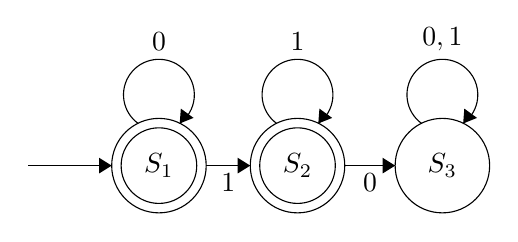
\begin{tikzpicture}[scale=0.2]
    \tikzstyle{every node}+=[inner sep=0pt]
    \draw [black] (23.7,-34.2) circle (3);
    \draw (23.7,-34.2) node {$S_1$};
    \draw [black] (23.7,-34.2) circle (2.4);
    \draw [black] (32.5,-34.2) circle (3);
    \draw (32.5,-34.2) node {$S_2$};
    \draw [black] (32.5,-34.2) circle (2.4);
    \draw [black] (41.7,-34.2) circle (3);
    \draw (41.7,-34.2) node {$S_3$};
    \draw [black] (15.4,-34.2) -- (20.7,-34.2);
    \fill [black] (20.7,-34.2) -- (19.9,-33.7) -- (19.9,-34.7);
    \draw [black] (26.7,-34.2) -- (29.5,-34.2);
    \fill [black] (29.5,-34.2) -- (28.7,-33.7) -- (28.7,-34.7);
    \draw (28.1,-34.7) node [below] {$1$};
    \draw [black] (31.177,-31.52) arc (234:-54:2.25);
    \draw (32.5,-26.95) node [above] {$1$};
    \fill [black] (33.82,-31.52) -- (34.7,-31.17) -- (33.89,-30.58);
    \draw [black] (22.377,-31.52) arc (234:-54:2.25);
    \draw (23.7,-26.95) node [above] {$0$};
    \fill [black] (25.02,-31.52) -- (25.9,-31.17) -- (25.09,-30.58);
    \draw [black] (35.5,-34.2) -- (38.7,-34.2);
    \fill [black] (38.7,-34.2) -- (37.9,-33.7) -- (37.9,-34.7);
    \draw (37.1,-34.7) node [below] {$0$};
    \draw [black] (40.377,-31.52) arc (234:-54:2.25);
    \draw (41.7,-26.95) node [above] {$0,1$};
    \fill [black] (43.02,-31.52) -- (43.9,-31.17) -- (43.09,-30.58);
    \end{tikzpicture}
    \end{center}

    Therefore the language, A, is regular.
    \end{proof}
	\item $B= \{ www \ | \ w \in \{0,1\}^* \}$
	\begin{proof}
        Assume B is regular. Let $p$ be the pumping length. Let $w = 0^p1^p0^p1^p0^p1^p$. If we were to remove any substring of $w$ by setting $i=0$ under the constraints of the pumping lemma ($xy^iz \in B$), we would end up with a string that is not in $B$ as it would not ever be symmetrical as the language implies.
        
        The same follows for the opposite. If we attempted to pump any substring of our string, we would end up with a string that is not in $B$ as it would not ever be symmetrical as the front half would be larger than the back half.
        
        We have found a contradiction according to the pumping lemma. Therefore, B is not regular.
    \end{proof}
\end{itemize}

\pagebreak

\problem{6} Find and describe the error that exists in the following proof. The proof attempts to show that $0^*1^*$ is not regular, when in fact it is:
\\
\\
\emph{
Assume, for sake of contradiction, that $0^*1^*$ is regular. We select an element from this language that is greater than the pumping length $p$. We select $0^p1^p$. In class, when proving that $0^n1^n$ was not regular, we showed that $0^p1^p$ cannot be pumped. Therefore, $0^*1^*$ is not regular.
}
\\
\\
In class, when we showed that $0^p1^p$ could not be pumped, it was under the constraint that there had to be an equal number of zeroes and ones. In the case of $0^*1^*$, there is no such constraint and we are free to pump any substring of the string.

In fact we can show this by the three cases of substrings that we can pump:

\begin{itemize}
    \item If we pump the leading zeroes, we will end up with a string that is still in the language.
    \item If we pump the lagging ones, we will end up with a string that is still in the language.
    \item If we pump some combination of the zeroes and ones, we will end up with a string that is still in the language.
\end{itemize}

Therefore, $0^*1^*$ is regular.

\end{document}
